\documentclass[sigconf]{acmart}

\usepackage{graphicx}
\graphicspath{ {./images/} }
\usepackage{caption}
\usepackage{subcaption}

% Meta information
\title{Image “Outpainting” and Hole Filling: Progress Report}
\subtitle{CS 5787 Deep Learning Final Project Milestone}

\author{Wentao Ye}
\email{wy335@cornell.edu}
\affiliation{%
  \institution{Cornell University}
}

\author{Mitchell Krieger}
\email{mak483@cornell.edu}
\affiliation{%
  \institution{Cornell University}
}

\author{Sebastian Jay}
\email{srj63@cornell.edu}
\affiliation{%
  \institution{Cornell University}
}

% Document begins
\begin{document}

\maketitle

\section*{Team Members}
Wentao Ye (wy335), Mitchell Krieger (mak483), Sebastian Jay (srj63)

\section*{Proposal}
Traditionally, image interpolation or inpainting tries to fill in a removed section of an image. There are a variety of methodologies for image interpolation, but our hope is to attempt a new approach where we can interpolate a scene between two disparate images by using image outpainting or image extrapolation. Outpainting or image extrapolation is the process of taking an image and generating an extension of the image beyond the original border. In general, outpainting is a difficult task because it requires the model to expand beyond a known region to generate scenes that look real. Our idea is to take two images and see if we can train a GAN-like architecture to outpaint these two images towards one another to complete a scene. We will be basing this project on the work done in \href{https://arxiv.org/abs/2201.11403}{Generalised Image Outpainting with U-Transformer by Gao et. al (2022) [LINK]}, which leveraged a transformer-based GAN they call a U-transformer. In the past, image outpainting only focused in the horizontal direction. However, in this paper, Gao et al, were able to outpaint horizontally and vertically. We hope to use this architecture to train a new GAN-based approach that can interpolate diagonally adjacent image gaps. This is different from interpolation in the past which was able to use the context of the surrounding image to fill in a removed section. Instead, our focus is on seeing if the model can understand how to connect different scenes in a realistic way. If successful, it means that the model understands relationships between disparate images and can model the visual world in a more precise way.

\section*{Datasets}
We used the \href{https://github.com/z-x-yang/NS-Outpainting}{NS-Outpainting [LINK]} dataset to train our models. It is used in the original U-Transformer paper. We also tested our trained model on additional images sourced from the internet.

\section*{Progress}

\subsection*{1. Reproduction of the paper}
Below is an example of what we were able to achieve within 20 epochs, to fill in an image using the original U-Transformer model. 

\begin{figure}[h]
    \centering
    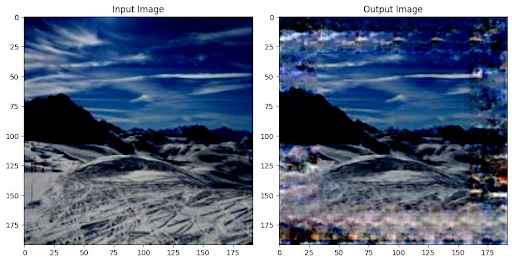
\includegraphics[width=0.8\linewidth]{utransformer.png}
    \caption{Image generated using U-Transformer after 20 epochs.}
\end{figure}

The U-transformer has the following shortcomings:
\begin{itemize}
    \item Fixed size 192
    \item Expensive, requires an NVIDIA A100 GPU in Google Colab to train.
    \item Slow, using an RTX 2070 takes 3 hours per epoch, i.e. 1500 hours for 500 epochs.
    \item Hard code in the Swintransformer model with the center logic so we have to update everything inside the model if we want to crop with different regions.
\end{itemize}

\subsection*{2. New GAN Solution}
The U-Transformer is based on Swin-transformer, which is quite slow, so we want to make it faster and cheaper.

Specifically, we use a GAN framework featuring a \href{https://paperswithcode.com/method/u-net-gan}{U-Net GAN generator [LINK]} and a \href{https://paperswithcode.com/method/patchgan}{PatchGAN discriminator [LINK]} for image outpainting and scene interpolation. The generator’s encoder-decoder with skip connections creates missing regions, while the discriminator evaluates patch realism. Training optimizes adversarial and reconstruction losses using the Adam optimizer, enabling seamless scene integration. Its benefits are as follows:
\begin{itemize}
    \item Fast, low memory usage, can run on a single RTX 2070
    \item It achieved the results shown below after 20 epochs, training for 3 hours
    \item 256 $\times$ 256 size
    \item \href{https://drive.google.com/file/d/1EORJGbg-rMQ_FNpzz7OSG73Vluro0Lxl/view?usp=sharing}{Weights [LINK]}
    \item \href{https://drive.google.com/drive/u/2/folders/1wOD_tgj9k3gUZI9hBL-WtKDS-uvz9m5S}{Code (Google Drive) [LINK]}
\end{itemize}

\begin{figure}[h]
    \centering
    \begin{subfigure}[b]{0.3\linewidth}
        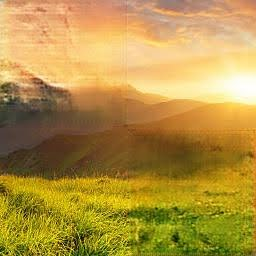
\includegraphics[width=\linewidth]{output1.jpg}
        \caption{Generated}
    \end{subfigure}
    \hfill
    \begin{subfigure}[b]{0.3\linewidth}
        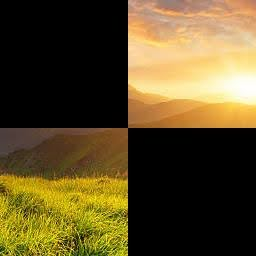
\includegraphics[width=\linewidth]{input1.jpg}
        \caption{Input}
    \end{subfigure}
    \hfill
    \begin{subfigure}[b]{0.3\linewidth}
        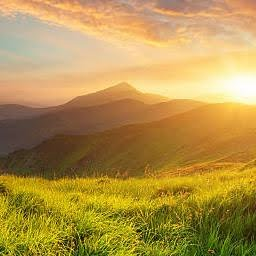
\includegraphics[width=\linewidth]{original1.jpg}
        \caption{Original}
    \end{subfigure}
    \caption{Results from the new GAN model (L-R: Generated, Input, Original).}
\end{figure}

\begin{figure}[h]
    \centering
    \begin{subfigure}[b]{0.3\linewidth}
        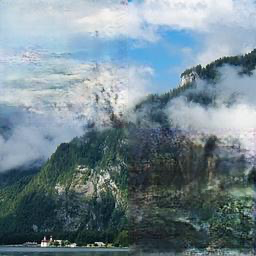
\includegraphics[width=\linewidth]{output2.png}
        \caption{Generated}
    \end{subfigure}
    \hfill
    \begin{subfigure}[b]{0.3\linewidth}
        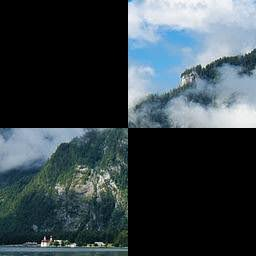
\includegraphics[width=\linewidth]{input2.jpg}
        \caption{Input}
    \end{subfigure}
    \hfill
    \begin{subfigure}[b]{0.3\linewidth}
        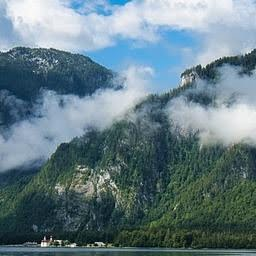
\includegraphics[width=\linewidth]{original2.jpg}
        \caption{Original}
    \end{subfigure}
    \caption{Results from the new GAN model (L-R: Generated, Input, Original).}
\end{figure}

\begin{figure}[h]
    \centering
    \begin{subfigure}[b]{0.3\linewidth}
        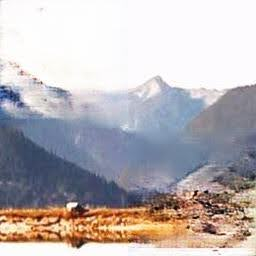
\includegraphics[width=\linewidth]{output3.jpg}
        \caption{Generated}
    \end{subfigure}
    \hfill
    \begin{subfigure}[b]{0.3\linewidth}
        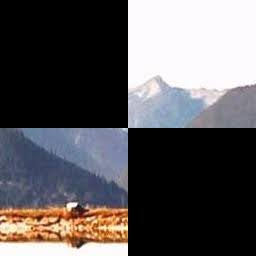
\includegraphics[width=\linewidth]{input3.jpg}
        \caption{Input}
    \end{subfigure}
    \hfill
    \begin{subfigure}[b]{0.3\linewidth}
        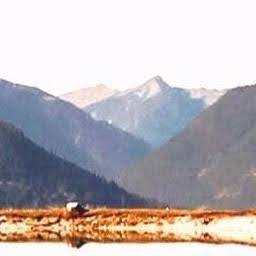
\includegraphics[width=\linewidth]{original3.jpg}
        \caption{Original}
    \end{subfigure}
    \caption{Results from the new GAN model (L-R: Generated, Input, Original).}
\end{figure}

\subsection*{3. New Diffusion Model}
In addition, we looked into additional papers that use diffusion models for tasks like this instead of GANs such as “RePaint: Inpainting using Denoising Diffusion Probabilistic Models” by Lugmayr et al (2022). Using this research we built an initial diffusion model that inpaints the NS-outpainiting dataset using diffusion. This model was trained on pairs of images and varying masks to represent unknown regions. In the training process, noise is gradually added to only the area where the masks are and MSE is used to attempt to predict this noise over 1000 timesteps. Then the diffusion model attempts to denoise only the pixels that are in the mask. After training for 14 epochs, the diffusion approach shows promising results.  

\begin{itemize}
    \item Trained on NVIDIA A100 in Google Colab, training took ~2.66 hours for 14 epochs
    \item 320 $\times$ 512 Image size
    \item \href{https://drive.google.com/file/d/1-wr7a01nVmRRFrYpwbjaQlc0FIDKINvY/view?usp=sharing}{Weights [LINK]}
    \item \href{https://colab.research.google.com/drive/1XZfe98Ox-r8rhJx-8WGiJiJjFm-hb6yO?authuser=2}{Code (Google Drive) [LINK]}
\end{itemize}

\begin{figure}[h]
    \centering
    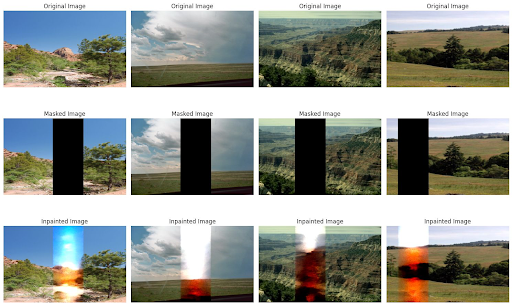
\includegraphics[width=0.8\linewidth]{diffusion_results.png}
    \caption{Original, masked, and inpainted images using diffusion model.}
\end{figure}

\section*{Next Steps}
We would like to train our model on more data, including on images from the RealEstate10K dataset. We’d like to figure out how to make our model predict only the missing parts of the image, rather than regenerating the entire image.

We will use the following metrics to evaluate our results:
\begin{itemize}
    \item \textbf{FID (Frechet Inception Distance)}: Assesses the similarity between the distributions of generated and real images, measuring both quality and diversity.
    \item \textbf{PSNR (Peak Signal-to-Noise Ratio)}: Evaluates the reconstruction quality by quantifying the pixel-level differences between generated and original images.
    \item \textbf{SSIM (Structural Similarity Index)}: Measures the structural similarity and perceptual quality between generated and ground truth images.
    \item \textbf{IS (Inception Score)}: Evaluates the clarity and diversity of generated images using a pre-trained Inception model.
\end{itemize}

\subsection*{Additional TODOs for GAN:}
\begin{itemize}
    \item Randomize location and size of cropped areas in training images (hard based on GAN)
    \item Bigger image size
    \item Smaller crop size
    \item Generate only the missing part, instead of using mask (hard based on GAN)
    \item Use two different images as each input sample
    \item Update loss function to optimize the performance
\end{itemize}

\subsection*{Additional TODOs for Diffusion:}
\begin{itemize}
    \item Train for additional epochs
    \item More masks of varying shapes
    \item Use Wasserstein Loss to better anchor generated inpaints to the original image, and penalize excess RGB color divergence in output image from input
    \item Better tune Gaussian Blur to make the boundary between the inpaint and the original model less stark.
\end{itemize}

\end{document}
